\section{Remoção}

\begin{frame}[fragile]{Remoção em árvores-B}

	Há 2 casos a serem tratados na remoção de uma chave em uma árvore-B, uma vez 
        localizado o nó onde deve ocorrer a remoção:

	\begin{enumerate}
		\item O nó é uma folha: 

		\begin{enumerate}
			\item Após a remoção da chave, restantam ainda $M = \lceil m/2\rceil - 1$ chaves ou
                mais

			\item Após a remoção da chave, a folha possui menos do que $M$ chaves 
                (\textit{underflow})

			\begin{enumerate}
				\item Se o irmão à direita ou à esquerda com mais do que $M$ chaves,
				as chaves são distribuídas entre o nó e seu irmão, passando a chave do pai para o 
                nó e a chave apropriada do irmão para o pai

				\item Se os irmãos à direita e à esquerda possuem o mínimo $M$ de
                    chaves, o nó é fundido com um de seus irmãos: as chaves do nó, a chave 
                    do pai e as chaves do irmão formam um novo nó, e o irmão é descartado
			\end{enumerate}

		\end{enumerate} 

		\item O nó é não é uma folha: este pode ser reduzido ao caso anterior trocando o elemento 
            a ser removido com seu sucessor (ou predecessor) que se encontra em uma folha
	\end{enumerate} 

\end{frame} 

\begin{frame}[fragile]{Exemplo de remoção no caso 1.1, $m = 4$}

    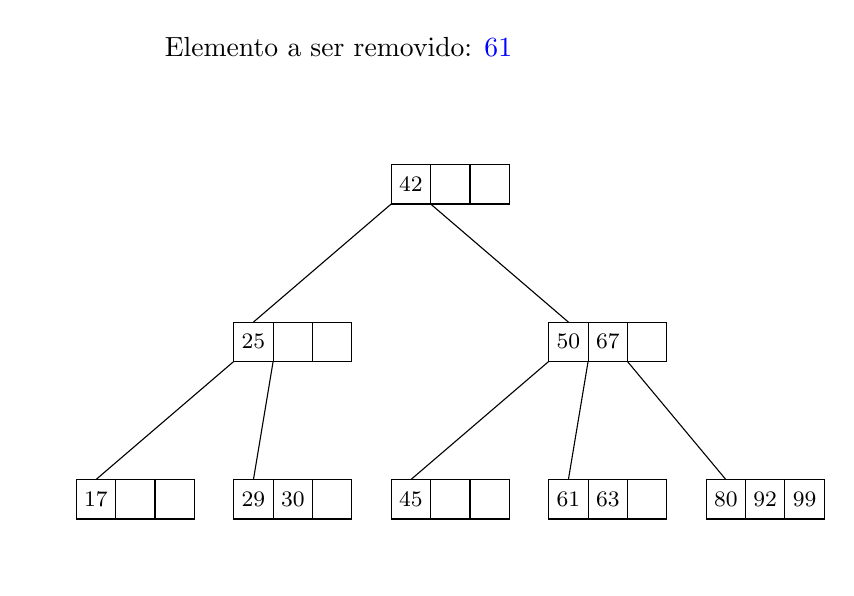
\begin{tikzpicture}
        \begin{scope}
            \node[opacity=0] at (-0.5, -0.5) { } ;
            \node[anchor=west] at (1, 6.0) { Elemento a ser removido: \textcolor{blue}{61} };

            \draw (4, 4) rectangle (4.5, 4.5);
            \draw (4.5, 4) rectangle (5, 4.5);
            \draw (5, 4) rectangle (5.5, 4.5);

            \draw (2, 2) rectangle (2.5, 2.5);
            \draw (2.5, 2) rectangle (3, 2.5);
            \draw (3, 2) rectangle (3.5, 2.5);

            \draw (6, 2) rectangle (6.5, 2.5);
            \draw (6.5, 2) rectangle (7, 2.5);
            \draw (7, 2) rectangle (7.5, 2.5);

            \draw (0, 0) rectangle (0.5, 0.5);
            \draw (0.5, 0) rectangle (1, 0.5);
            \draw (1, 0) rectangle (1.5, 0.5);

            \draw (2, 0) rectangle (2.5, 0.5);
            \draw (2.5, 0) rectangle (3, 0.5);
            \draw (3, 0) rectangle (3.5, 0.5);

            \draw (4, 0) rectangle (4.5, 0.5);
            \draw (4.5, 0) rectangle (5, 0.5);
            \draw (5, 0) rectangle (5.5, 0.5);

            \draw (6, 0) rectangle (6.5, 0.5);
            \draw (6.5, 0) rectangle (7, 0.5);
            \draw (7, 0) rectangle (7.5, 0.5);

            \draw (8, 0) rectangle (8.5, 0.5);
            \draw (8.5, 0) rectangle (9, 0.5);
            \draw (9, 0) rectangle (9.5, 0.5);

            \node at (4.25, 4.25) { \footnotesize \textcolor{black}{42} };

            \node at (2.25, 2.25) { \footnotesize \textcolor{black}{25} };

            \node at (6.25, 2.25) { \footnotesize \textcolor{black}{50} };
            \node at (6.75, 2.25) { \footnotesize \textcolor{black}{67} };

            \node at (0.25, 0.25) { \footnotesize \textcolor{black}{17} };

            \node at (2.25, 0.25) { \footnotesize \textcolor{black}{29} };
            \node at (2.75, 0.25) { \footnotesize \textcolor{black}{30} };

            \node at (4.25, 0.25) { \footnotesize \textcolor{black}{45} };

            \node at (6.25, 0.25) { \footnotesize \textcolor{black}{61} };
            \node at (6.75, 0.25) { \footnotesize \textcolor{black}{63} };

            \node at (8.25, 0.25) { \footnotesize \textcolor{black}{80} };
            \node at (8.75, 0.25) { \footnotesize \textcolor{black}{92} };
            \node at (9.25, 0.25) { \footnotesize \textcolor{black}{99} };

            \draw (4,4) -- (2.25, 2.5);
            \draw (4.5,4) -- (6.25, 2.5);
            \draw (7,2) -- (8.25, 0.5);

            \draw (2,2) -- (0.25, 0.5);
            \draw (2.5,2) -- (2.25, 0.5);
            \draw (6,2) -- (4.25, 0.5);
            \draw (6.5,2) -- (6.25, 0.5);

        \end{scope}
 
    \end{tikzpicture}
\end{frame}


\begin{frame}[fragile]{Exemplo de remoção no caso 1.1, $m = 4$}

    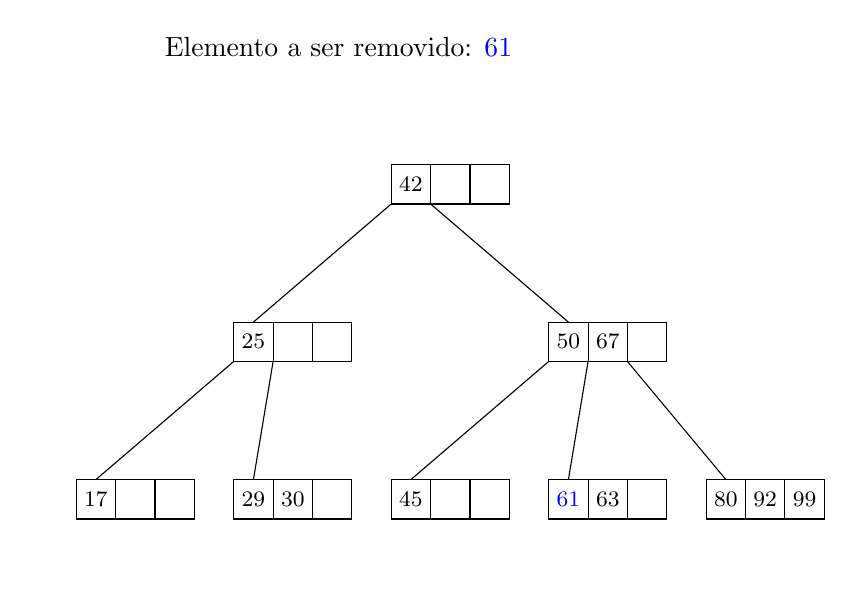
\begin{tikzpicture}
        \begin{scope}
            \node[opacity=0] at (-0.5, -0.5) { } ;
            \node[anchor=west] at (1, 6.0) { Elemento a ser removido: \textcolor{blue}{61} };

            \draw (4, 4) rectangle (4.5, 4.5);
            \draw (4.5, 4) rectangle (5, 4.5);
            \draw (5, 4) rectangle (5.5, 4.5);

            \draw (2, 2) rectangle (2.5, 2.5);
            \draw (2.5, 2) rectangle (3, 2.5);
            \draw (3, 2) rectangle (3.5, 2.5);

            \draw (6, 2) rectangle (6.5, 2.5);
            \draw (6.5, 2) rectangle (7, 2.5);
            \draw (7, 2) rectangle (7.5, 2.5);

            \draw (0, 0) rectangle (0.5, 0.5);
            \draw (0.5, 0) rectangle (1, 0.5);
            \draw (1, 0) rectangle (1.5, 0.5);

            \draw (2, 0) rectangle (2.5, 0.5);
            \draw (2.5, 0) rectangle (3, 0.5);
            \draw (3, 0) rectangle (3.5, 0.5);

            \draw (4, 0) rectangle (4.5, 0.5);
            \draw (4.5, 0) rectangle (5, 0.5);
            \draw (5, 0) rectangle (5.5, 0.5);

            \draw (6, 0) rectangle (6.5, 0.5);
            \draw (6.5, 0) rectangle (7, 0.5);
            \draw (7, 0) rectangle (7.5, 0.5);

            \draw (8, 0) rectangle (8.5, 0.5);
            \draw (8.5, 0) rectangle (9, 0.5);
            \draw (9, 0) rectangle (9.5, 0.5);

            \node at (4.25, 4.25) { \footnotesize \textcolor{black}{42} };

            \node at (2.25, 2.25) { \footnotesize \textcolor{black}{25} };

            \node at (6.25, 2.25) { \footnotesize \textcolor{black}{50} };
            \node at (6.75, 2.25) { \footnotesize \textcolor{black}{67} };

            \node at (0.25, 0.25) { \footnotesize \textcolor{black}{17} };

            \node at (2.25, 0.25) { \footnotesize \textcolor{black}{29} };
            \node at (2.75, 0.25) { \footnotesize \textcolor{black}{30} };

            \node at (4.25, 0.25) { \footnotesize \textcolor{black}{45} };

            \node at (6.25, 0.25) { \footnotesize \textcolor{blue}{61} };
            \node at (6.75, 0.25) { \footnotesize \textcolor{black}{63} };

            \node at (8.25, 0.25) { \footnotesize \textcolor{black}{80} };
            \node at (8.75, 0.25) { \footnotesize \textcolor{black}{92} };
            \node at (9.25, 0.25) { \footnotesize \textcolor{black}{99} };

            \draw (4,4) -- (2.25, 2.5);
            \draw (4.5,4) -- (6.25, 2.5);
            \draw (7,2) -- (8.25, 0.5);

            \draw (2,2) -- (0.25, 0.5);
            \draw (2.5,2) -- (2.25, 0.5);
            \draw (6,2) -- (4.25, 0.5);
            \draw (6.5,2) -- (6.25, 0.5);

        \end{scope}
 
    \end{tikzpicture}
\end{frame}

\begin{frame}[fragile]{Exemplo de remoção no caso 1.1, $m = 4$}

    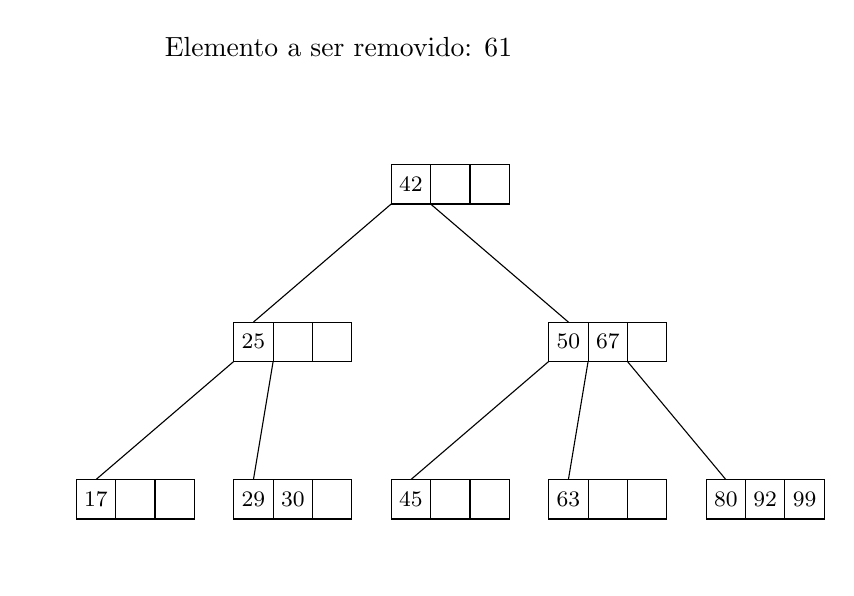
\begin{tikzpicture}
        \begin{scope}
            \node[opacity=0] at (-0.5, -0.5) { } ;
            \node[anchor=west] at (1, 6.0) { Elemento a ser removido: \textcolor{black}{61} };

            \draw (4, 4) rectangle (4.5, 4.5);
            \draw (4.5, 4) rectangle (5, 4.5);
            \draw (5, 4) rectangle (5.5, 4.5);

            \draw (2, 2) rectangle (2.5, 2.5);
            \draw (2.5, 2) rectangle (3, 2.5);
            \draw (3, 2) rectangle (3.5, 2.5);

            \draw (6, 2) rectangle (6.5, 2.5);
            \draw (6.5, 2) rectangle (7, 2.5);
            \draw (7, 2) rectangle (7.5, 2.5);

            \draw (0, 0) rectangle (0.5, 0.5);
            \draw (0.5, 0) rectangle (1, 0.5);
            \draw (1, 0) rectangle (1.5, 0.5);

            \draw (2, 0) rectangle (2.5, 0.5);
            \draw (2.5, 0) rectangle (3, 0.5);
            \draw (3, 0) rectangle (3.5, 0.5);

            \draw (4, 0) rectangle (4.5, 0.5);
            \draw (4.5, 0) rectangle (5, 0.5);
            \draw (5, 0) rectangle (5.5, 0.5);

            \draw (6, 0) rectangle (6.5, 0.5);
            \draw (6.5, 0) rectangle (7, 0.5);
            \draw (7, 0) rectangle (7.5, 0.5);

            \draw (8, 0) rectangle (8.5, 0.5);
            \draw (8.5, 0) rectangle (9, 0.5);
            \draw (9, 0) rectangle (9.5, 0.5);

            \node at (4.25, 4.25) { \footnotesize \textcolor{black}{42} };

            \node at (2.25, 2.25) { \footnotesize \textcolor{black}{25} };

            \node at (6.25, 2.25) { \footnotesize \textcolor{black}{50} };
            \node at (6.75, 2.25) { \footnotesize \textcolor{black}{67} };

            \node at (0.25, 0.25) { \footnotesize \textcolor{black}{17} };

            \node at (2.25, 0.25) { \footnotesize \textcolor{black}{29} };
            \node at (2.75, 0.25) { \footnotesize \textcolor{black}{30} };

            \node at (4.25, 0.25) { \footnotesize \textcolor{black}{45} };

            \node at (6.25, 0.25) { \footnotesize \textcolor{black}{63} };

            \node at (8.25, 0.25) { \footnotesize \textcolor{black}{80} };
            \node at (8.75, 0.25) { \footnotesize \textcolor{black}{92} };
            \node at (9.25, 0.25) { \footnotesize \textcolor{black}{99} };

            \draw (4,4) -- (2.25, 2.5);
            \draw (4.5,4) -- (6.25, 2.5);
            \draw (7,2) -- (8.25, 0.5);

            \draw (2,2) -- (0.25, 0.5);
            \draw (2.5,2) -- (2.25, 0.5);
            \draw (6,2) -- (4.25, 0.5);
            \draw (6.5,2) -- (6.25, 0.5);

        \end{scope}
 
    \end{tikzpicture}
\end{frame}

\begin{frame}[fragile]{Exemplo de remoção no caso 1.2.1, $m = 4$}

    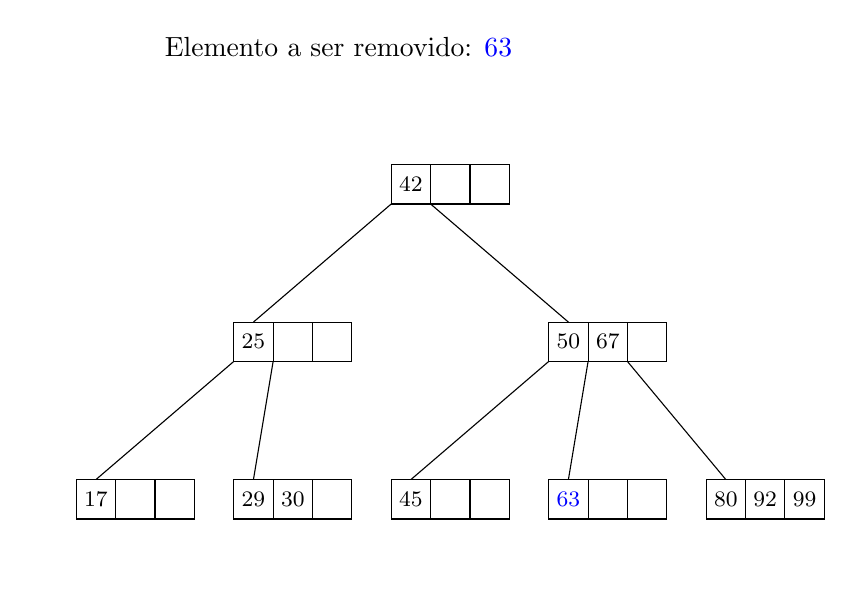
\begin{tikzpicture}
        \begin{scope}
            \node[opacity=0] at (-0.5, -0.5) { } ;
            \node[anchor=west] at (1, 6.0) { Elemento a ser removido: \textcolor{blue}{63} };

            \draw (4, 4) rectangle (4.5, 4.5);
            \draw (4.5, 4) rectangle (5, 4.5);
            \draw (5, 4) rectangle (5.5, 4.5);

            \draw (2, 2) rectangle (2.5, 2.5);
            \draw (2.5, 2) rectangle (3, 2.5);
            \draw (3, 2) rectangle (3.5, 2.5);

            \draw (6, 2) rectangle (6.5, 2.5);
            \draw (6.5, 2) rectangle (7, 2.5);
            \draw (7, 2) rectangle (7.5, 2.5);

            \draw (0, 0) rectangle (0.5, 0.5);
            \draw (0.5, 0) rectangle (1, 0.5);
            \draw (1, 0) rectangle (1.5, 0.5);

            \draw (2, 0) rectangle (2.5, 0.5);
            \draw (2.5, 0) rectangle (3, 0.5);
            \draw (3, 0) rectangle (3.5, 0.5);

            \draw (4, 0) rectangle (4.5, 0.5);
            \draw (4.5, 0) rectangle (5, 0.5);
            \draw (5, 0) rectangle (5.5, 0.5);

            \draw (6, 0) rectangle (6.5, 0.5);
            \draw (6.5, 0) rectangle (7, 0.5);
            \draw (7, 0) rectangle (7.5, 0.5);

            \draw (8, 0) rectangle (8.5, 0.5);
            \draw (8.5, 0) rectangle (9, 0.5);
            \draw (9, 0) rectangle (9.5, 0.5);

            \node at (4.25, 4.25) { \footnotesize \textcolor{black}{42} };

            \node at (2.25, 2.25) { \footnotesize \textcolor{black}{25} };

            \node at (6.25, 2.25) { \footnotesize \textcolor{black}{50} };
            \node at (6.75, 2.25) { \footnotesize \textcolor{black}{67} };

            \node at (0.25, 0.25) { \footnotesize \textcolor{black}{17} };

            \node at (2.25, 0.25) { \footnotesize \textcolor{black}{29} };
            \node at (2.75, 0.25) { \footnotesize \textcolor{black}{30} };

            \node at (4.25, 0.25) { \footnotesize \textcolor{black}{45} };

            \node at (6.25, 0.25) { \footnotesize \textcolor{blue}{63} };

            \node at (8.25, 0.25) { \footnotesize \textcolor{black}{80} };
            \node at (8.75, 0.25) { \footnotesize \textcolor{black}{92} };
            \node at (9.25, 0.25) { \footnotesize \textcolor{black}{99} };

            \draw (4,4) -- (2.25, 2.5);
            \draw (4.5,4) -- (6.25, 2.5);
            \draw (7,2) -- (8.25, 0.5);

            \draw (2,2) -- (0.25, 0.5);
            \draw (2.5,2) -- (2.25, 0.5);
            \draw (6,2) -- (4.25, 0.5);
            \draw (6.5,2) -- (6.25, 0.5);

        \end{scope}
 
    \end{tikzpicture}
\end{frame}

\begin{frame}[fragile]{Exemplo de remoção no caso 1.2.1, $m = 4$}

    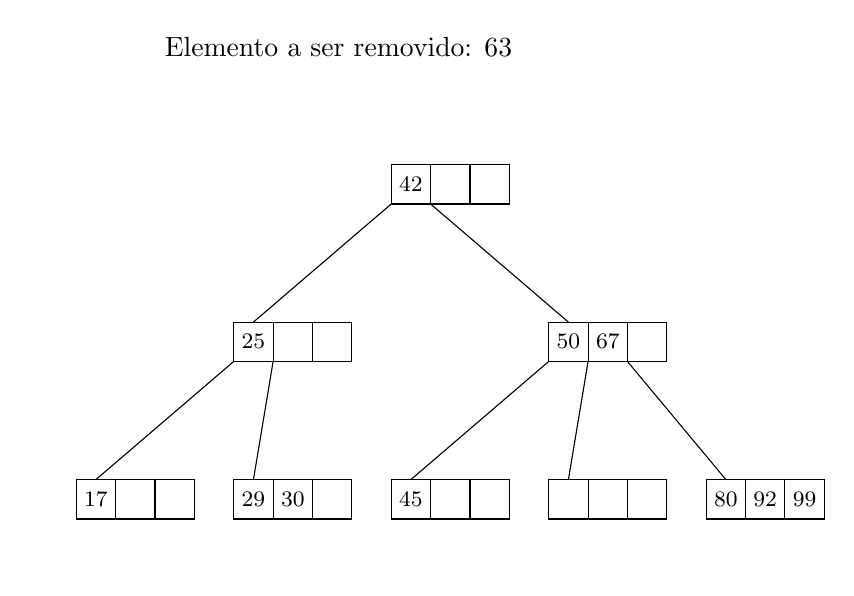
\begin{tikzpicture}
        \begin{scope}
            \node[opacity=0] at (-0.5, -0.5) { } ;
            \node[anchor=west] at (1, 6.0) { Elemento a ser removido: \textcolor{black}{63} };

            \draw (4, 4) rectangle (4.5, 4.5);
            \draw (4.5, 4) rectangle (5, 4.5);
            \draw (5, 4) rectangle (5.5, 4.5);

            \draw (2, 2) rectangle (2.5, 2.5);
            \draw (2.5, 2) rectangle (3, 2.5);
            \draw (3, 2) rectangle (3.5, 2.5);

            \draw (6, 2) rectangle (6.5, 2.5);
            \draw (6.5, 2) rectangle (7, 2.5);
            \draw (7, 2) rectangle (7.5, 2.5);

            \draw (0, 0) rectangle (0.5, 0.5);
            \draw (0.5, 0) rectangle (1, 0.5);
            \draw (1, 0) rectangle (1.5, 0.5);

            \draw (2, 0) rectangle (2.5, 0.5);
            \draw (2.5, 0) rectangle (3, 0.5);
            \draw (3, 0) rectangle (3.5, 0.5);

            \draw (4, 0) rectangle (4.5, 0.5);
            \draw (4.5, 0) rectangle (5, 0.5);
            \draw (5, 0) rectangle (5.5, 0.5);

            \draw (6, 0) rectangle (6.5, 0.5);
            \draw (6.5, 0) rectangle (7, 0.5);
            \draw (7, 0) rectangle (7.5, 0.5);

            \draw (8, 0) rectangle (8.5, 0.5);
            \draw (8.5, 0) rectangle (9, 0.5);
            \draw (9, 0) rectangle (9.5, 0.5);

            \node at (4.25, 4.25) { \footnotesize \textcolor{black}{42} };

            \node at (2.25, 2.25) { \footnotesize \textcolor{black}{25} };

            \node at (6.25, 2.25) { \footnotesize \textcolor{black}{50} };
            \node at (6.75, 2.25) { \footnotesize \textcolor{black}{67} };

            \node at (0.25, 0.25) { \footnotesize \textcolor{black}{17} };

            \node at (2.25, 0.25) { \footnotesize \textcolor{black}{29} };
            \node at (2.75, 0.25) { \footnotesize \textcolor{black}{30} };

            \node at (4.25, 0.25) { \footnotesize \textcolor{black}{45} };

            \node at (8.25, 0.25) { \footnotesize \textcolor{black}{80} };
            \node at (8.75, 0.25) { \footnotesize \textcolor{black}{92} };
            \node at (9.25, 0.25) { \footnotesize \textcolor{black}{99} };

            \draw (4,4) -- (2.25, 2.5);
            \draw (4.5,4) -- (6.25, 2.5);
            \draw (7,2) -- (8.25, 0.5);

            \draw (2,2) -- (0.25, 0.5);
            \draw (2.5,2) -- (2.25, 0.5);
            \draw (6,2) -- (4.25, 0.5);
            \draw (6.5,2) -- (6.25, 0.5);

        \end{scope}
 
    \end{tikzpicture}
\end{frame}

\begin{frame}[fragile]{Exemplo de remoção no caso 1.2.1, $m = 4$}

    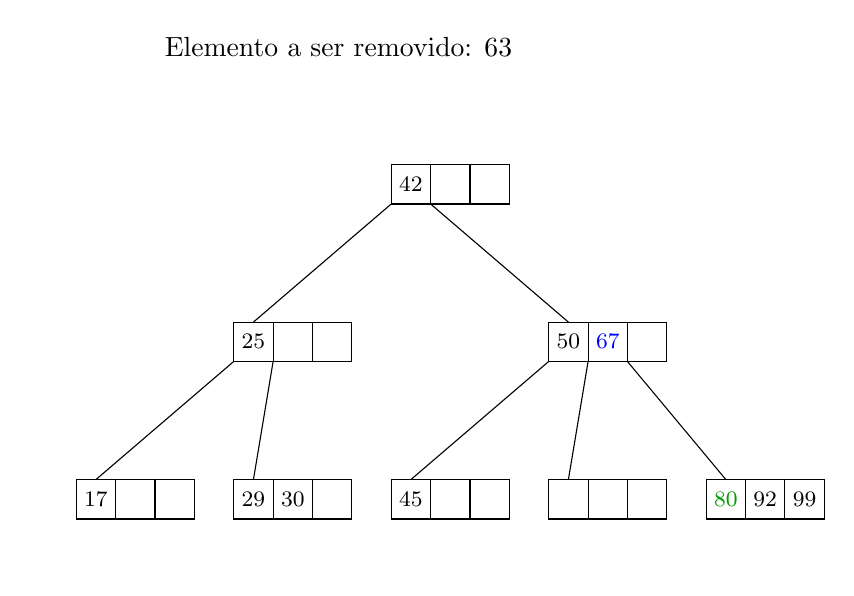
\begin{tikzpicture}
        \begin{scope}
            \node[opacity=0] at (-0.5, -0.5) { } ;
            \node[anchor=west] at (1, 6.0) { Elemento a ser removido: \textcolor{black}{63} };

            \draw (4, 4) rectangle (4.5, 4.5);
            \draw (4.5, 4) rectangle (5, 4.5);
            \draw (5, 4) rectangle (5.5, 4.5);

            \draw (2, 2) rectangle (2.5, 2.5);
            \draw (2.5, 2) rectangle (3, 2.5);
            \draw (3, 2) rectangle (3.5, 2.5);

            \draw (6, 2) rectangle (6.5, 2.5);
            \draw (6.5, 2) rectangle (7, 2.5);
            \draw (7, 2) rectangle (7.5, 2.5);

            \draw (0, 0) rectangle (0.5, 0.5);
            \draw (0.5, 0) rectangle (1, 0.5);
            \draw (1, 0) rectangle (1.5, 0.5);

            \draw (2, 0) rectangle (2.5, 0.5);
            \draw (2.5, 0) rectangle (3, 0.5);
            \draw (3, 0) rectangle (3.5, 0.5);

            \draw (4, 0) rectangle (4.5, 0.5);
            \draw (4.5, 0) rectangle (5, 0.5);
            \draw (5, 0) rectangle (5.5, 0.5);

            \draw (6, 0) rectangle (6.5, 0.5);
            \draw (6.5, 0) rectangle (7, 0.5);
            \draw (7, 0) rectangle (7.5, 0.5);

            \draw (8, 0) rectangle (8.5, 0.5);
            \draw (8.5, 0) rectangle (9, 0.5);
            \draw (9, 0) rectangle (9.5, 0.5);

            \node at (4.25, 4.25) { \footnotesize \textcolor{black}{42} };

            \node at (2.25, 2.25) { \footnotesize \textcolor{black}{25} };

            \node at (6.25, 2.25) { \footnotesize \textcolor{black}{50} };
            \node at (6.75, 2.25) { \footnotesize \textcolor{blue}{67} };

            \node at (0.25, 0.25) { \footnotesize \textcolor{black}{17} };

            \node at (2.25, 0.25) { \footnotesize \textcolor{black}{29} };
            \node at (2.75, 0.25) { \footnotesize \textcolor{black}{30} };

            \node at (4.25, 0.25) { \footnotesize \textcolor{black}{45} };

            \node at (8.25, 0.25) { \footnotesize \textcolor{green!60!black}{80} };
            \node at (8.75, 0.25) { \footnotesize \textcolor{black}{92} };
            \node at (9.25, 0.25) { \footnotesize \textcolor{black}{99} };

            \draw (4,4) -- (2.25, 2.5);
            \draw (4.5,4) -- (6.25, 2.5);
            \draw (7,2) -- (8.25, 0.5);

            \draw (2,2) -- (0.25, 0.5);
            \draw (2.5,2) -- (2.25, 0.5);
            \draw (6,2) -- (4.25, 0.5);
            \draw (6.5,2) -- (6.25, 0.5);

        \end{scope}
 
    \end{tikzpicture}
\end{frame}

\begin{frame}[fragile]{Exemplo de remoção no caso 1.2.1, $m = 4$}

    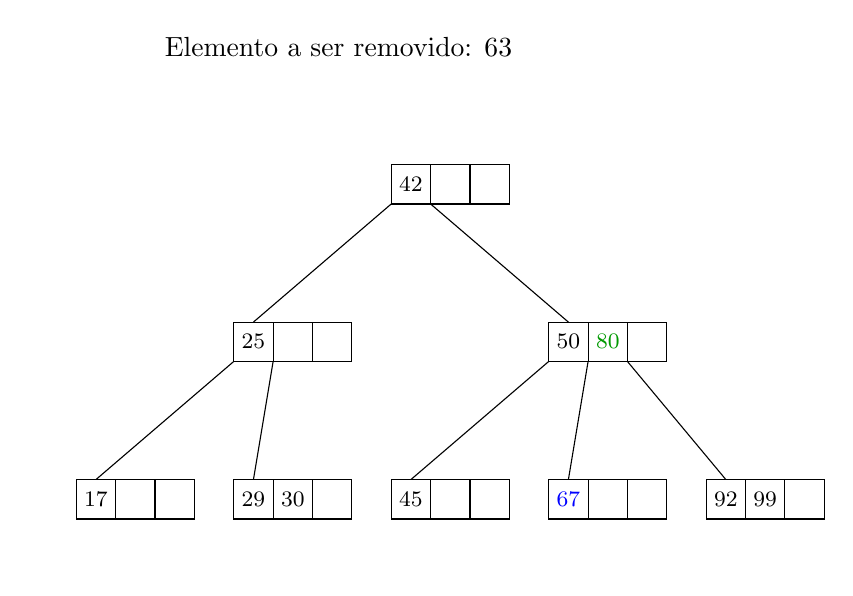
\begin{tikzpicture}
        \begin{scope}
            \node[opacity=0] at (-0.5, -0.5) { } ;
            \node[anchor=west] at (1, 6.0) { Elemento a ser removido: \textcolor{black}{63} };

            \draw (4, 4) rectangle (4.5, 4.5);
            \draw (4.5, 4) rectangle (5, 4.5);
            \draw (5, 4) rectangle (5.5, 4.5);

            \draw (2, 2) rectangle (2.5, 2.5);
            \draw (2.5, 2) rectangle (3, 2.5);
            \draw (3, 2) rectangle (3.5, 2.5);

            \draw (6, 2) rectangle (6.5, 2.5);
            \draw (6.5, 2) rectangle (7, 2.5);
            \draw (7, 2) rectangle (7.5, 2.5);

            \draw (0, 0) rectangle (0.5, 0.5);
            \draw (0.5, 0) rectangle (1, 0.5);
            \draw (1, 0) rectangle (1.5, 0.5);

            \draw (2, 0) rectangle (2.5, 0.5);
            \draw (2.5, 0) rectangle (3, 0.5);
            \draw (3, 0) rectangle (3.5, 0.5);

            \draw (4, 0) rectangle (4.5, 0.5);
            \draw (4.5, 0) rectangle (5, 0.5);
            \draw (5, 0) rectangle (5.5, 0.5);

            \draw (6, 0) rectangle (6.5, 0.5);
            \draw (6.5, 0) rectangle (7, 0.5);
            \draw (7, 0) rectangle (7.5, 0.5);

            \draw (8, 0) rectangle (8.5, 0.5);
            \draw (8.5, 0) rectangle (9, 0.5);
            \draw (9, 0) rectangle (9.5, 0.5);

            \node at (4.25, 4.25) { \footnotesize \textcolor{black}{42} };

            \node at (2.25, 2.25) { \footnotesize \textcolor{black}{25} };

            \node at (6.25, 2.25) { \footnotesize \textcolor{black}{50} };
            \node at (6.75, 2.25) { \footnotesize \textcolor{green!60!black}{80} };

            \node at (0.25, 0.25) { \footnotesize \textcolor{black}{17} };

            \node at (2.25, 0.25) { \footnotesize \textcolor{black}{29} };
            \node at (2.75, 0.25) { \footnotesize \textcolor{black}{30} };

            \node at (4.25, 0.25) { \footnotesize \textcolor{black}{45} };

            \node at (6.25, 0.25) { \footnotesize \textcolor{blue}{67} };

            \node at (8.25, 0.25) { \footnotesize \textcolor{black}{92} };
            \node at (8.75, 0.25) { \footnotesize \textcolor{black}{99} };

            \draw (4,4) -- (2.25, 2.5);
            \draw (4.5,4) -- (6.25, 2.5);
            \draw (7,2) -- (8.25, 0.5);

            \draw (2,2) -- (0.25, 0.5);
            \draw (2.5,2) -- (2.25, 0.5);
            \draw (6,2) -- (4.25, 0.5);
            \draw (6.5,2) -- (6.25, 0.5);

        \end{scope}
 
    \end{tikzpicture}
\end{frame}

\begin{frame}[fragile]{Exemplo de remoção no caso 1.2.2, $m = 4$}

    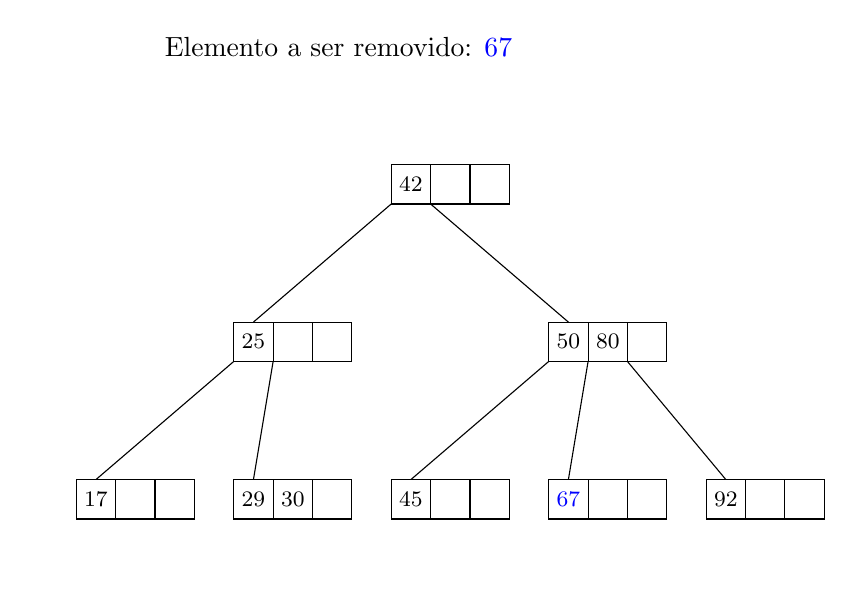
\begin{tikzpicture}
        \begin{scope}
            \node[opacity=0] at (-0.5, -0.5) { } ;
            \node[anchor=west] at (1, 6.0) { Elemento a ser removido: \textcolor{blue}{67} };

            \draw (4, 4) rectangle (4.5, 4.5);
            \draw (4.5, 4) rectangle (5, 4.5);
            \draw (5, 4) rectangle (5.5, 4.5);

            \draw (2, 2) rectangle (2.5, 2.5);
            \draw (2.5, 2) rectangle (3, 2.5);
            \draw (3, 2) rectangle (3.5, 2.5);

            \draw (6, 2) rectangle (6.5, 2.5);
            \draw (6.5, 2) rectangle (7, 2.5);
            \draw (7, 2) rectangle (7.5, 2.5);

            \draw (0, 0) rectangle (0.5, 0.5);
            \draw (0.5, 0) rectangle (1, 0.5);
            \draw (1, 0) rectangle (1.5, 0.5);

            \draw (2, 0) rectangle (2.5, 0.5);
            \draw (2.5, 0) rectangle (3, 0.5);
            \draw (3, 0) rectangle (3.5, 0.5);

            \draw (4, 0) rectangle (4.5, 0.5);
            \draw (4.5, 0) rectangle (5, 0.5);
            \draw (5, 0) rectangle (5.5, 0.5);

            \draw (6, 0) rectangle (6.5, 0.5);
            \draw (6.5, 0) rectangle (7, 0.5);
            \draw (7, 0) rectangle (7.5, 0.5);

            \draw (8, 0) rectangle (8.5, 0.5);
            \draw (8.5, 0) rectangle (9, 0.5);
            \draw (9, 0) rectangle (9.5, 0.5);

            \node at (4.25, 4.25) { \footnotesize \textcolor{black}{42} };

            \node at (2.25, 2.25) { \footnotesize \textcolor{black}{25} };

            \node at (6.25, 2.25) { \footnotesize \textcolor{black}{50} };
            \node at (6.75, 2.25) { \footnotesize \textcolor{black}{80} };

            \node at (0.25, 0.25) { \footnotesize \textcolor{black}{17} };

            \node at (2.25, 0.25) { \footnotesize \textcolor{black}{29} };
            \node at (2.75, 0.25) { \footnotesize \textcolor{black}{30} };

            \node at (4.25, 0.25) { \footnotesize \textcolor{black}{45} };

            \node at (6.25, 0.25) { \footnotesize \textcolor{blue}{67} };

            \node at (8.25, 0.25) { \footnotesize \textcolor{black}{92} };

            \draw (4,4) -- (2.25, 2.5);
            \draw (4.5,4) -- (6.25, 2.5);
            \draw (7,2) -- (8.25, 0.5);

            \draw (2,2) -- (0.25, 0.5);
            \draw (2.5,2) -- (2.25, 0.5);
            \draw (6,2) -- (4.25, 0.5);
            \draw (6.5,2) -- (6.25, 0.5);

        \end{scope}
 
    \end{tikzpicture}
\end{frame}

\begin{frame}[fragile]{Exemplo de remoção no caso 1.2.2, $m = 4$}

    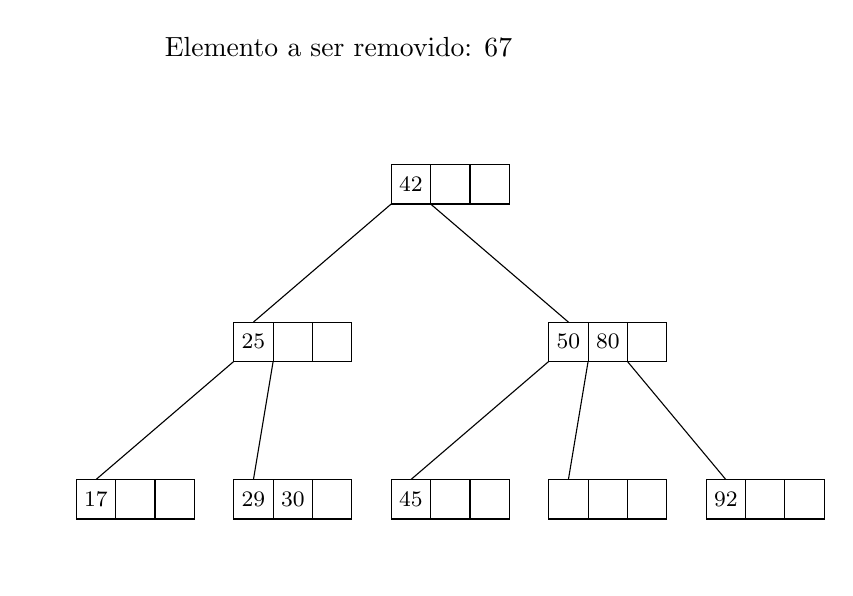
\begin{tikzpicture}
        \begin{scope}
            \node[opacity=0] at (-0.5, -0.5) { } ;
            \node[anchor=west] at (1, 6.0) { Elemento a ser removido: \textcolor{black}{67} };

            \draw (4, 4) rectangle (4.5, 4.5);
            \draw (4.5, 4) rectangle (5, 4.5);
            \draw (5, 4) rectangle (5.5, 4.5);

            \draw (2, 2) rectangle (2.5, 2.5);
            \draw (2.5, 2) rectangle (3, 2.5);
            \draw (3, 2) rectangle (3.5, 2.5);

            \draw (6, 2) rectangle (6.5, 2.5);
            \draw (6.5, 2) rectangle (7, 2.5);
            \draw (7, 2) rectangle (7.5, 2.5);

            \draw (0, 0) rectangle (0.5, 0.5);
            \draw (0.5, 0) rectangle (1, 0.5);
            \draw (1, 0) rectangle (1.5, 0.5);

            \draw (2, 0) rectangle (2.5, 0.5);
            \draw (2.5, 0) rectangle (3, 0.5);
            \draw (3, 0) rectangle (3.5, 0.5);

            \draw (4, 0) rectangle (4.5, 0.5);
            \draw (4.5, 0) rectangle (5, 0.5);
            \draw (5, 0) rectangle (5.5, 0.5);

            \draw (6, 0) rectangle (6.5, 0.5);
            \draw (6.5, 0) rectangle (7, 0.5);
            \draw (7, 0) rectangle (7.5, 0.5);

            \draw (8, 0) rectangle (8.5, 0.5);
            \draw (8.5, 0) rectangle (9, 0.5);
            \draw (9, 0) rectangle (9.5, 0.5);

            \node at (4.25, 4.25) { \footnotesize \textcolor{black}{42} };

            \node at (2.25, 2.25) { \footnotesize \textcolor{black}{25} };

            \node at (6.25, 2.25) { \footnotesize \textcolor{black}{50} };
            \node at (6.75, 2.25) { \footnotesize \textcolor{black}{80} };

            \node at (0.25, 0.25) { \footnotesize \textcolor{black}{17} };

            \node at (2.25, 0.25) { \footnotesize \textcolor{black}{29} };
            \node at (2.75, 0.25) { \footnotesize \textcolor{black}{30} };

            \node at (4.25, 0.25) { \footnotesize \textcolor{black}{45} };

%            \node at (6.25, 0.25) { \footnotesize \textcolor{blue}{67} };

            \node at (8.25, 0.25) { \footnotesize \textcolor{black}{92} };

            \draw (4,4) -- (2.25, 2.5);
            \draw (4.5,4) -- (6.25, 2.5);
            \draw (7,2) -- (8.25, 0.5);

            \draw (2,2) -- (0.25, 0.5);
            \draw (2.5,2) -- (2.25, 0.5);
            \draw (6,2) -- (4.25, 0.5);
            \draw (6.5,2) -- (6.25, 0.5);

        \end{scope}
 
    \end{tikzpicture}
\end{frame}

\begin{frame}[fragile]{Exemplo de remoção no caso 1.2.2, $m = 4$}

    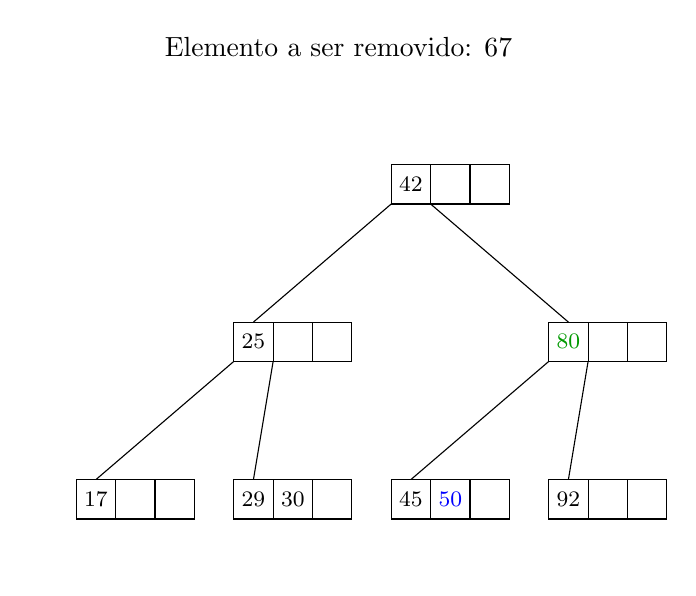
\begin{tikzpicture}
        \begin{scope}
            \node[opacity=0] at (-0.5, -0.5) { } ;
            \node[anchor=west] at (1, 6.0) { Elemento a ser removido: \textcolor{black}{67} };

            \draw (4, 4) rectangle (4.5, 4.5);
            \draw (4.5, 4) rectangle (5, 4.5);
            \draw (5, 4) rectangle (5.5, 4.5);

            \draw (2, 2) rectangle (2.5, 2.5);
            \draw (2.5, 2) rectangle (3, 2.5);
            \draw (3, 2) rectangle (3.5, 2.5);

            \draw (6, 2) rectangle (6.5, 2.5);
            \draw (6.5, 2) rectangle (7, 2.5);
            \draw (7, 2) rectangle (7.5, 2.5);

            \draw (0, 0) rectangle (0.5, 0.5);
            \draw (0.5, 0) rectangle (1, 0.5);
            \draw (1, 0) rectangle (1.5, 0.5);

            \draw (2, 0) rectangle (2.5, 0.5);
            \draw (2.5, 0) rectangle (3, 0.5);
            \draw (3, 0) rectangle (3.5, 0.5);

            \draw (4, 0) rectangle (4.5, 0.5);
            \draw (4.5, 0) rectangle (5, 0.5);
            \draw (5, 0) rectangle (5.5, 0.5);

            \draw (6, 0) rectangle (6.5, 0.5);
            \draw (6.5, 0) rectangle (7, 0.5);
            \draw (7, 0) rectangle (7.5, 0.5);

%            \draw (8, 0) rectangle (8.5, 0.5);
%            \draw (8.5, 0) rectangle (9, 0.5);
%            \draw (9, 0) rectangle (9.5, 0.5);

            \node at (4.25, 4.25) { \footnotesize \textcolor{black}{42} };

            \node at (2.25, 2.25) { \footnotesize \textcolor{black}{25} };

            \node at (6.25, 2.25) { \footnotesize \textcolor{green!60!black}{80} };
%            \node at (6.75, 2.25) { \footnotesize \textcolor{black}{80} };

            \node at (0.25, 0.25) { \footnotesize \textcolor{black}{17} };

            \node at (2.25, 0.25) { \footnotesize \textcolor{black}{29} };
            \node at (2.75, 0.25) { \footnotesize \textcolor{black}{30} };

            \node at (4.25, 0.25) { \footnotesize \textcolor{black}{45} };
            \node at (4.75, 0.25) { \footnotesize \textcolor{blue}{50} };

            \node at (6.25, 0.25) { \footnotesize \textcolor{black}{92} };

%            \node at (8.25, 0.25) { \footnotesize \textcolor{black}{92} };

            \draw (4,4) -- (2.25, 2.5);
            \draw (4.5,4) -- (6.25, 2.5);
%            \draw (7,2) -- (8.25, 0.5);

            \draw (2,2) -- (0.25, 0.5);
            \draw (2.5,2) -- (2.25, 0.5);
            \draw (6,2) -- (4.25, 0.5);
            \draw (6.5,2) -- (6.25, 0.5);

        \end{scope}
 
    \end{tikzpicture}
\end{frame}

\begin{frame}[fragile]{Exemplo de remoção no caso 2, $m = 4$}

    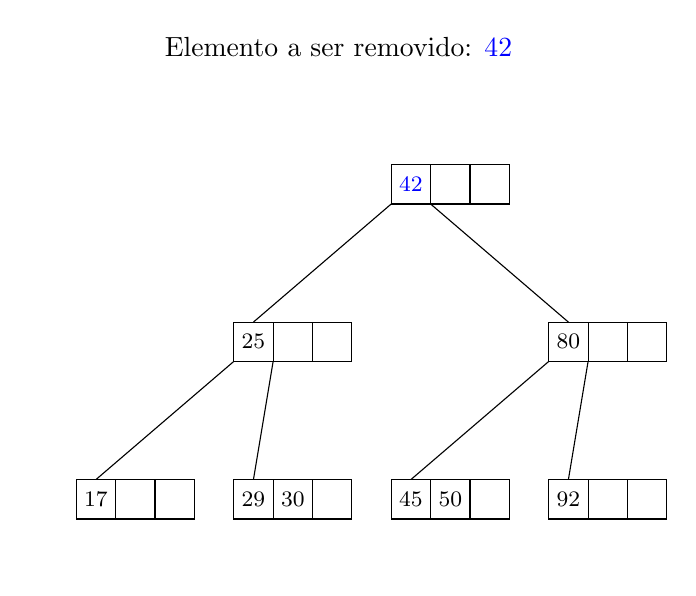
\begin{tikzpicture}
        \begin{scope}
            \node[opacity=0] at (-0.5, -0.5) { } ;
            \node[anchor=west] at (1, 6.0) { Elemento a ser removido: \textcolor{blue}{42} };

            \draw (4, 4) rectangle (4.5, 4.5);
            \draw (4.5, 4) rectangle (5, 4.5);
            \draw (5, 4) rectangle (5.5, 4.5);

            \draw (2, 2) rectangle (2.5, 2.5);
            \draw (2.5, 2) rectangle (3, 2.5);
            \draw (3, 2) rectangle (3.5, 2.5);

            \draw (6, 2) rectangle (6.5, 2.5);
            \draw (6.5, 2) rectangle (7, 2.5);
            \draw (7, 2) rectangle (7.5, 2.5);

            \draw (0, 0) rectangle (0.5, 0.5);
            \draw (0.5, 0) rectangle (1, 0.5);
            \draw (1, 0) rectangle (1.5, 0.5);

            \draw (2, 0) rectangle (2.5, 0.5);
            \draw (2.5, 0) rectangle (3, 0.5);
            \draw (3, 0) rectangle (3.5, 0.5);

            \draw (4, 0) rectangle (4.5, 0.5);
            \draw (4.5, 0) rectangle (5, 0.5);
            \draw (5, 0) rectangle (5.5, 0.5);

            \draw (6, 0) rectangle (6.5, 0.5);
            \draw (6.5, 0) rectangle (7, 0.5);
            \draw (7, 0) rectangle (7.5, 0.5);

            \node at (4.25, 4.25) { \footnotesize \textcolor{blue}{42} };

            \node at (2.25, 2.25) { \footnotesize \textcolor{black}{25} };

            \node at (6.25, 2.25) { \footnotesize \textcolor{black}{80} };

            \node at (0.25, 0.25) { \footnotesize \textcolor{black}{17} };

            \node at (2.25, 0.25) { \footnotesize \textcolor{black}{29} };
            \node at (2.75, 0.25) { \footnotesize \textcolor{black}{30} };

            \node at (4.25, 0.25) { \footnotesize \textcolor{black}{45} };
            \node at (4.75, 0.25) { \footnotesize \textcolor{black}{50} };

            \node at (6.25, 0.25) { \footnotesize \textcolor{black}{92} };

            \draw (4,4) -- (2.25, 2.5);
            \draw (4.5,4) -- (6.25, 2.5);

            \draw (2,2) -- (0.25, 0.5);
            \draw (2.5,2) -- (2.25, 0.5);
            \draw (6,2) -- (4.25, 0.5);
            \draw (6.5,2) -- (6.25, 0.5);

        \end{scope}
 
    \end{tikzpicture}
\end{frame}

\begin{frame}[fragile]{Exemplo de remoção no caso 2, $m = 4$}

    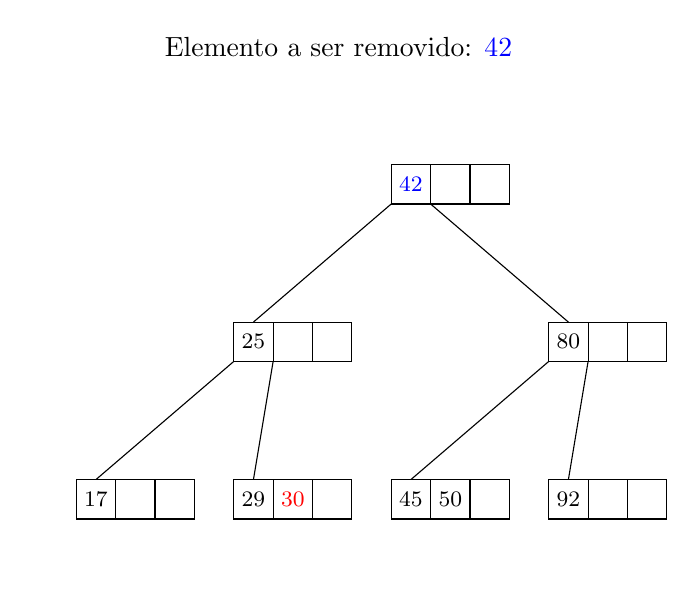
\begin{tikzpicture}
        \begin{scope}
            \node[opacity=0] at (-0.5, -0.5) { } ;
            \node[anchor=west] at (1, 6.0) { Elemento a ser removido: \textcolor{blue}{42} };

            \draw (4, 4) rectangle (4.5, 4.5);
            \draw (4.5, 4) rectangle (5, 4.5);
            \draw (5, 4) rectangle (5.5, 4.5);

            \draw (2, 2) rectangle (2.5, 2.5);
            \draw (2.5, 2) rectangle (3, 2.5);
            \draw (3, 2) rectangle (3.5, 2.5);

            \draw (6, 2) rectangle (6.5, 2.5);
            \draw (6.5, 2) rectangle (7, 2.5);
            \draw (7, 2) rectangle (7.5, 2.5);

            \draw (0, 0) rectangle (0.5, 0.5);
            \draw (0.5, 0) rectangle (1, 0.5);
            \draw (1, 0) rectangle (1.5, 0.5);

            \draw (2, 0) rectangle (2.5, 0.5);
            \draw (2.5, 0) rectangle (3, 0.5);
            \draw (3, 0) rectangle (3.5, 0.5);

            \draw (4, 0) rectangle (4.5, 0.5);
            \draw (4.5, 0) rectangle (5, 0.5);
            \draw (5, 0) rectangle (5.5, 0.5);

            \draw (6, 0) rectangle (6.5, 0.5);
            \draw (6.5, 0) rectangle (7, 0.5);
            \draw (7, 0) rectangle (7.5, 0.5);

            \node at (4.25, 4.25) { \footnotesize \textcolor{blue}{42} };

            \node at (2.25, 2.25) { \footnotesize \textcolor{black}{25} };

            \node at (6.25, 2.25) { \footnotesize \textcolor{black}{80} };

            \node at (0.25, 0.25) { \footnotesize \textcolor{black}{17} };

            \node at (2.25, 0.25) { \footnotesize \textcolor{black}{29} };
            \node at (2.75, 0.25) { \footnotesize \textcolor{red}{30} };

            \node at (4.25, 0.25) { \footnotesize \textcolor{black}{45} };
            \node at (4.75, 0.25) { \footnotesize \textcolor{black}{50} };

            \node at (6.25, 0.25) { \footnotesize \textcolor{black}{92} };

            \draw (4,4) -- (2.25, 2.5);
            \draw (4.5,4) -- (6.25, 2.5);

            \draw (2,2) -- (0.25, 0.5);
            \draw (2.5,2) -- (2.25, 0.5);
            \draw (6,2) -- (4.25, 0.5);
            \draw (6.5,2) -- (6.25, 0.5);

        \end{scope}
 
    \end{tikzpicture}
\end{frame}

\begin{frame}[fragile]{Exemplo de remoção no caso 2, $m = 4$}

    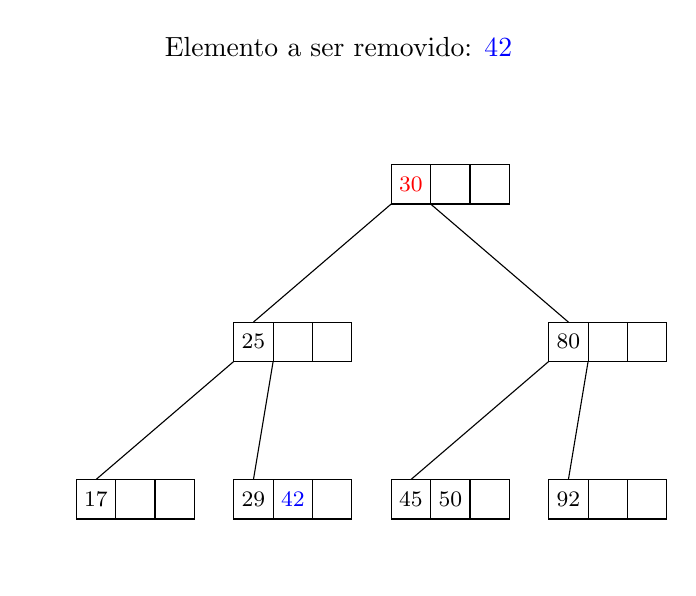
\begin{tikzpicture}
        \begin{scope}
            \node[opacity=0] at (-0.5, -0.5) { } ;
            \node[anchor=west] at (1, 6.0) { Elemento a ser removido: \textcolor{blue}{42} };

            \draw (4, 4) rectangle (4.5, 4.5);
            \draw (4.5, 4) rectangle (5, 4.5);
            \draw (5, 4) rectangle (5.5, 4.5);

            \draw (2, 2) rectangle (2.5, 2.5);
            \draw (2.5, 2) rectangle (3, 2.5);
            \draw (3, 2) rectangle (3.5, 2.5);

            \draw (6, 2) rectangle (6.5, 2.5);
            \draw (6.5, 2) rectangle (7, 2.5);
            \draw (7, 2) rectangle (7.5, 2.5);

            \draw (0, 0) rectangle (0.5, 0.5);
            \draw (0.5, 0) rectangle (1, 0.5);
            \draw (1, 0) rectangle (1.5, 0.5);

            \draw (2, 0) rectangle (2.5, 0.5);
            \draw (2.5, 0) rectangle (3, 0.5);
            \draw (3, 0) rectangle (3.5, 0.5);

            \draw (4, 0) rectangle (4.5, 0.5);
            \draw (4.5, 0) rectangle (5, 0.5);
            \draw (5, 0) rectangle (5.5, 0.5);

            \draw (6, 0) rectangle (6.5, 0.5);
            \draw (6.5, 0) rectangle (7, 0.5);
            \draw (7, 0) rectangle (7.5, 0.5);

            \node at (4.25, 4.25) { \footnotesize \textcolor{red}{30} };

            \node at (2.25, 2.25) { \footnotesize \textcolor{black}{25} };

            \node at (6.25, 2.25) { \footnotesize \textcolor{black}{80} };

            \node at (0.25, 0.25) { \footnotesize \textcolor{black}{17} };

            \node at (2.25, 0.25) { \footnotesize \textcolor{black}{29} };
            \node at (2.75, 0.25) { \footnotesize \textcolor{blue}{42} };

            \node at (4.25, 0.25) { \footnotesize \textcolor{black}{45} };
            \node at (4.75, 0.25) { \footnotesize \textcolor{black}{50} };

            \node at (6.25, 0.25) { \footnotesize \textcolor{black}{92} };

            \draw (4,4) -- (2.25, 2.5);
            \draw (4.5,4) -- (6.25, 2.5);

            \draw (2,2) -- (0.25, 0.5);
            \draw (2.5,2) -- (2.25, 0.5);
            \draw (6,2) -- (4.25, 0.5);
            \draw (6.5,2) -- (6.25, 0.5);

        \end{scope}
 
    \end{tikzpicture}
\end{frame}

\begin{frame}[fragile]{Exemplo de remoção no caso 2, $m = 4$}

    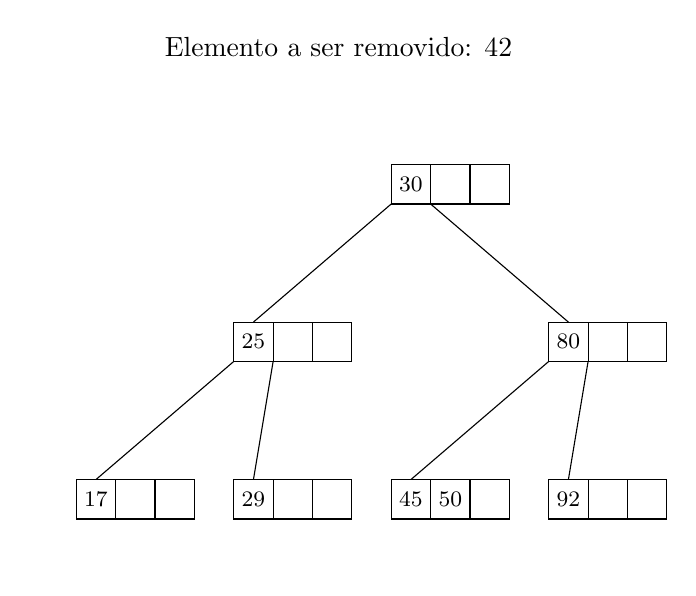
\begin{tikzpicture}
        \begin{scope}
            \node[opacity=0] at (-0.5, -0.5) { } ;
            \node[anchor=west] at (1, 6.0) { Elemento a ser removido: \textcolor{black}{42} };

            \draw (4, 4) rectangle (4.5, 4.5);
            \draw (4.5, 4) rectangle (5, 4.5);
            \draw (5, 4) rectangle (5.5, 4.5);

            \draw (2, 2) rectangle (2.5, 2.5);
            \draw (2.5, 2) rectangle (3, 2.5);
            \draw (3, 2) rectangle (3.5, 2.5);

            \draw (6, 2) rectangle (6.5, 2.5);
            \draw (6.5, 2) rectangle (7, 2.5);
            \draw (7, 2) rectangle (7.5, 2.5);

            \draw (0, 0) rectangle (0.5, 0.5);
            \draw (0.5, 0) rectangle (1, 0.5);
            \draw (1, 0) rectangle (1.5, 0.5);

            \draw (2, 0) rectangle (2.5, 0.5);
            \draw (2.5, 0) rectangle (3, 0.5);
            \draw (3, 0) rectangle (3.5, 0.5);

            \draw (4, 0) rectangle (4.5, 0.5);
            \draw (4.5, 0) rectangle (5, 0.5);
            \draw (5, 0) rectangle (5.5, 0.5);

            \draw (6, 0) rectangle (6.5, 0.5);
            \draw (6.5, 0) rectangle (7, 0.5);
            \draw (7, 0) rectangle (7.5, 0.5);

            \node at (4.25, 4.25) { \footnotesize \textcolor{black}{30} };

            \node at (2.25, 2.25) { \footnotesize \textcolor{black}{25} };

            \node at (6.25, 2.25) { \footnotesize \textcolor{black}{80} };

            \node at (0.25, 0.25) { \footnotesize \textcolor{black}{17} };

            \node at (2.25, 0.25) { \footnotesize \textcolor{black}{29} };

            \node at (4.25, 0.25) { \footnotesize \textcolor{black}{45} };
            \node at (4.75, 0.25) { \footnotesize \textcolor{black}{50} };

            \node at (6.25, 0.25) { \footnotesize \textcolor{black}{92} };

            \draw (4,4) -- (2.25, 2.5);
            \draw (4.5,4) -- (6.25, 2.5);

            \draw (2,2) -- (0.25, 0.5);
            \draw (2.5,2) -- (2.25, 0.5);
            \draw (6,2) -- (4.25, 0.5);
            \draw (6.5,2) -- (6.25, 0.5);

        \end{scope}
 
    \end{tikzpicture}
\end{frame}

\begin{frame}[fragile]{Implementação da remoção em uma árvore-B}
    \inputsnippet{cpp}{150}{170}{btree.cpp}
\end{frame}

\begin{frame}[fragile]{Implementação da remoção em uma árvore-B}
    \inputsnippet{cpp}{172}{192}{btree.cpp}
\end{frame}

\begin{frame}[fragile]{Implementação da remoção em uma árvore-B}
    \inputsnippet{cpp}{194}{214}{btree.cpp}
\end{frame}

\begin{frame}[fragile]{Implementação da remoção em uma árvore-B}
    \inputsnippet{cpp}{216}{236}{btree.cpp}
\end{frame}

\begin{frame}[fragile]{Implementação da remoção em uma árvore-B}
    \inputsnippet{cpp}{237}{255}{btree.cpp}
\end{frame}
